\section{Material y métodos}

Para llevar a cabo este trabajo, se utilizó un Macbook Pro (13 pulgadas, 
2020) equipado con el chip Apple M1 y memoria RAM de 16 GB, operando bajo el
sistema operativo macOS Ventura versión 13.3.1.

Los programas y bases de datos empleados en este trabajo quedan detallados 
en las \textbf{Tablas 1} y \textbf{2}.

\begin{table}[htbp]
    \centering
    \caption{Programas utilizados en sus versiones para macOS}\label{tab:programs}
    \scriptsize
    \setlength{\tabcolsep}{20pt}
    \begin{tabularx}{\textwidth}{@{}p{3cm}p{3cm}X@{}}
    \toprule
    \textbf{Nombre} & \textbf{Referencia} & \textbf{Acceso} \\ 
    \midrule
    MAFFT v7.490 & \cite{katoh_mafft_2013} & \url{https://mafft.cbrc.jp/alignment/software/} \\
    trimAl v1.4 & \cite{capella-gutierrez_trimal_2009} & \url{https://github.com/inab/trimal} \\
    IQ-TREE v2.2.0 & \cite{minh_iq-tree_2020} & \url{http://www.iqtree.org/} \\
    FigTree v1.4.4 & \cite{rambaut_figtree_2007} & \url{https://github.com/rambaut/figtree/releases} \\
    Jalview v2.11.2.6 & \cite{waterhouse_jalview_2009} & \url{https://www.jalview.org/} \\
    WebLogo v3.7.12 & \cite{crooks_weblogo_2004} & \url{https://weblogo.threeplusone.com/create.cgi} \\
    ChimeraX v1.6 & \cite{pettersen_span_2021} & \url{https://www.rbvi.ucsf.edu/chimerax/} \\
    Adobe Illustrator v27.0 & \cite{adobe_inc_adobe_2023} & \url{https://www.adobe.com/es/products} \\ 
    \bottomrule
    \end{tabularx}
\end{table}

\begin{table}[htbp]
    \centering
    \caption{Bases de datos en línea}\label{tab:databases}
    \scriptsize
    \setlength{\tabcolsep}{20pt} % Reduce el espacio entre columnas
    \begin{tabularx}{\textwidth}{@{}p{4.5cm}p{3cm}X@{}}
    \toprule
    \textbf{Nombre} & \textbf{Referencia} & \textbf{Acceso} \\
    \midrule
    National Center for Biotechnology Information (NCBI) & \cite{sayers_database_2023} & \url{https://www.ncbi.nlm.nih.gov/} \\
    GenBank & \cite{benson_genbank_2013} & \url{https://www.ncbi.nlm.nih.gov/genbank/} \\
    Protein Data Bank (PDB) & \cite{berman_protein_2000} & \url{https://www.rcsb.org/} \\
    The database of the International Committee on Taxonomy of Viruses (ICTV) & \cite{lefkowitz_virus_2018} & \url{https://ictv.global/} \\
    \bottomrule
    \end{tabularx}
\end{table}

\subsection{Análisis de secuencias aminoacídicas}

\subsubsection{Búsqueda y selección de secuencias}

El último informe del grupo de estudio del ICTV responsable de la familia
\textit{Coronaviridae} incluye los listados de especies reconocidas dentro 
de cada género, así como el acceso a un genoma de referencia para cada una 
dentro del GenBank (\cite{woo_family_2023}). En base a ello, se procedió a 
la descarga manual de las secuencias aminoacídicas correspondientes a las 
proteínas nsp10, nsp14 y nsp16 de todas las especies pertenecientes a la 
subfamilia Orthocoronavirinae. Adicionalmente, fueron incluidas las del 
único representante de la subfamilia \textit{Pitovirinae} para su uso como 
especie externa en alineamientos y filogenias. El representante de la 
subfamilia \textit{Letovirinae} fue descartado debido a que solo constaba 
una secuencia parcial de su genoma.

Cabe recordar que dentro de la especie Severe acute respiratory 
syndrome-related coronavirus existen virus diferenciados en base a su 
elevada relevancia clínica, como es el caso del SARS-CoV y el SARS-CoV-2, y 
es por lo que sus secuencias fueron añadidas al informe del ICTV y se 
incluyen en este trabajo. El listado completo de las especies utilizadas se 
adjunta en la \textbf{Tabla A1}.

Los métodos utilizados en este trabajo para el análisis de secuencias se 
ejemplificaron a partir de nsp10, pero también se aplicaron de manera 
similar a nsp14 y nsp16.

\subsubsection{Formato y organización de las secuencias}

Todas las secuencias aminoacídicas fueron descargadas como ficheros de texto
formato FASTA (.fasta). Con el objetivo de trabajar con las secuencias 
obtenidas utilizando otras herramientas, fue necesario concatenarlas en un 
único archivo. Para ello, se utilizó el siguiente comando en la terminal de 
macOS:\@

\begin{lstlisting}[language=bash]
 cat * >> ALL_NSP10.fasta 
\end{lstlisting}

El comando significa concatenar (\lstinline!cat!) el contenido de todos los 
archivos (\lstinline!*!) de la carpeta en la que se trabaja y redirigirlos 
(\lstinline!>>!) a uno nuevo (\lstinline!ALL_NSP10.fasta!). Este 
procedimiento permite agrupar las secuencias, generando un único documento 
FASTA para cada una de las familias de proteínas nsp10.

\subsubsection{Alineamiento de secuencias}

Se realizó la alineación múltiple de las secuencias biológicas mediante 
MAFFT en la terminal de macOS, el cual ofrece múltiples estrategias para 
llevar a cabo el proceso de alineación. En este caso se consideró que el 
dominio completo de cada familia de proteínas puede alinearse globalmente, 
por lo que se ejecutó el siguiente comando:

\begin{lstlisting}[language=bash]
 Mafft --globalpair --maxiterate 1000 ALL_NSP10.fasta > ALN_ALL_NSP10.fasta
\end{lstlisting}

Este comando ejecuta el programa (\lstinline!Mafft!) y establece que las 
secuencias deben ser alineadas globalmente en toda su extensión 
(\lstinline!--globalpair!), utilizando 1000 iteraciones 
(\lstinline!--maxiterate 1000!) para refinar el alineamiento. El archivo de 
entrada utilizado contiene las secuencias a alinear 
(\lstinline!ALL_NSP10.fasta!) y el resultado final se exporta 
(\lstinline!>!) a un nuevo archivo (\lstinline!ALN_ALL_NSP10.fasta!).

\subsubsection{Optimización de los alineamientos}

Los alineamientos obtenidos fueron depurados con TrimAl, una herramienta
bioinformática que permite mejorar la calidad de los alineamientos múltiples
y aumentar de este modo la confiabilidad de los análisis filogenéticos. Se 
utilizó a través de la terminal de macOS mediante el siguiente comando:

\begin{lstlisting}[language=bash]
 trimal -automated1 -in ALN_ALL_NSP10.fasta -out TRIM_ALN_ALL_NSP10.fasta -htmlout ALN_ALL_NSP10.html
\end{lstlisting}
    
Este comando ejecuta el programa (\lstinline!trimal!) usando un método 
heurístico enfocado en optimización de alineamientos que serán utilizados 
para la inferencia de árboles filogenéticos por métodos de máxima 
verosimilitud (\lstinline!-automated1!). A partir de un archivo de entrada 
(\lstinline!-in ALN_ALL_NSP10.fasta!) se obtiene otro de salida con el 
alineamiento ya optimizado (\lstinline!-out TRIM_ALN_ALL_NSP10.fasta!) 
así como un informe en formato HTML (\textit{HyperText Markup Language}) del 
proceso de depuración (\lstinline!-htmlout ALN_ALL_NSP10.html!). El informe 
utiliza el esquema de colores del programa Clustal X (\cite{thompson_clustal_x_1997}) 
(\textbf{Tabla A2}), el cual facilita poder evaluar los alineamientos y
detectar posibles problemas (\textbf{Figura 4}).

\begin{figure}[!ht]
    \centering
    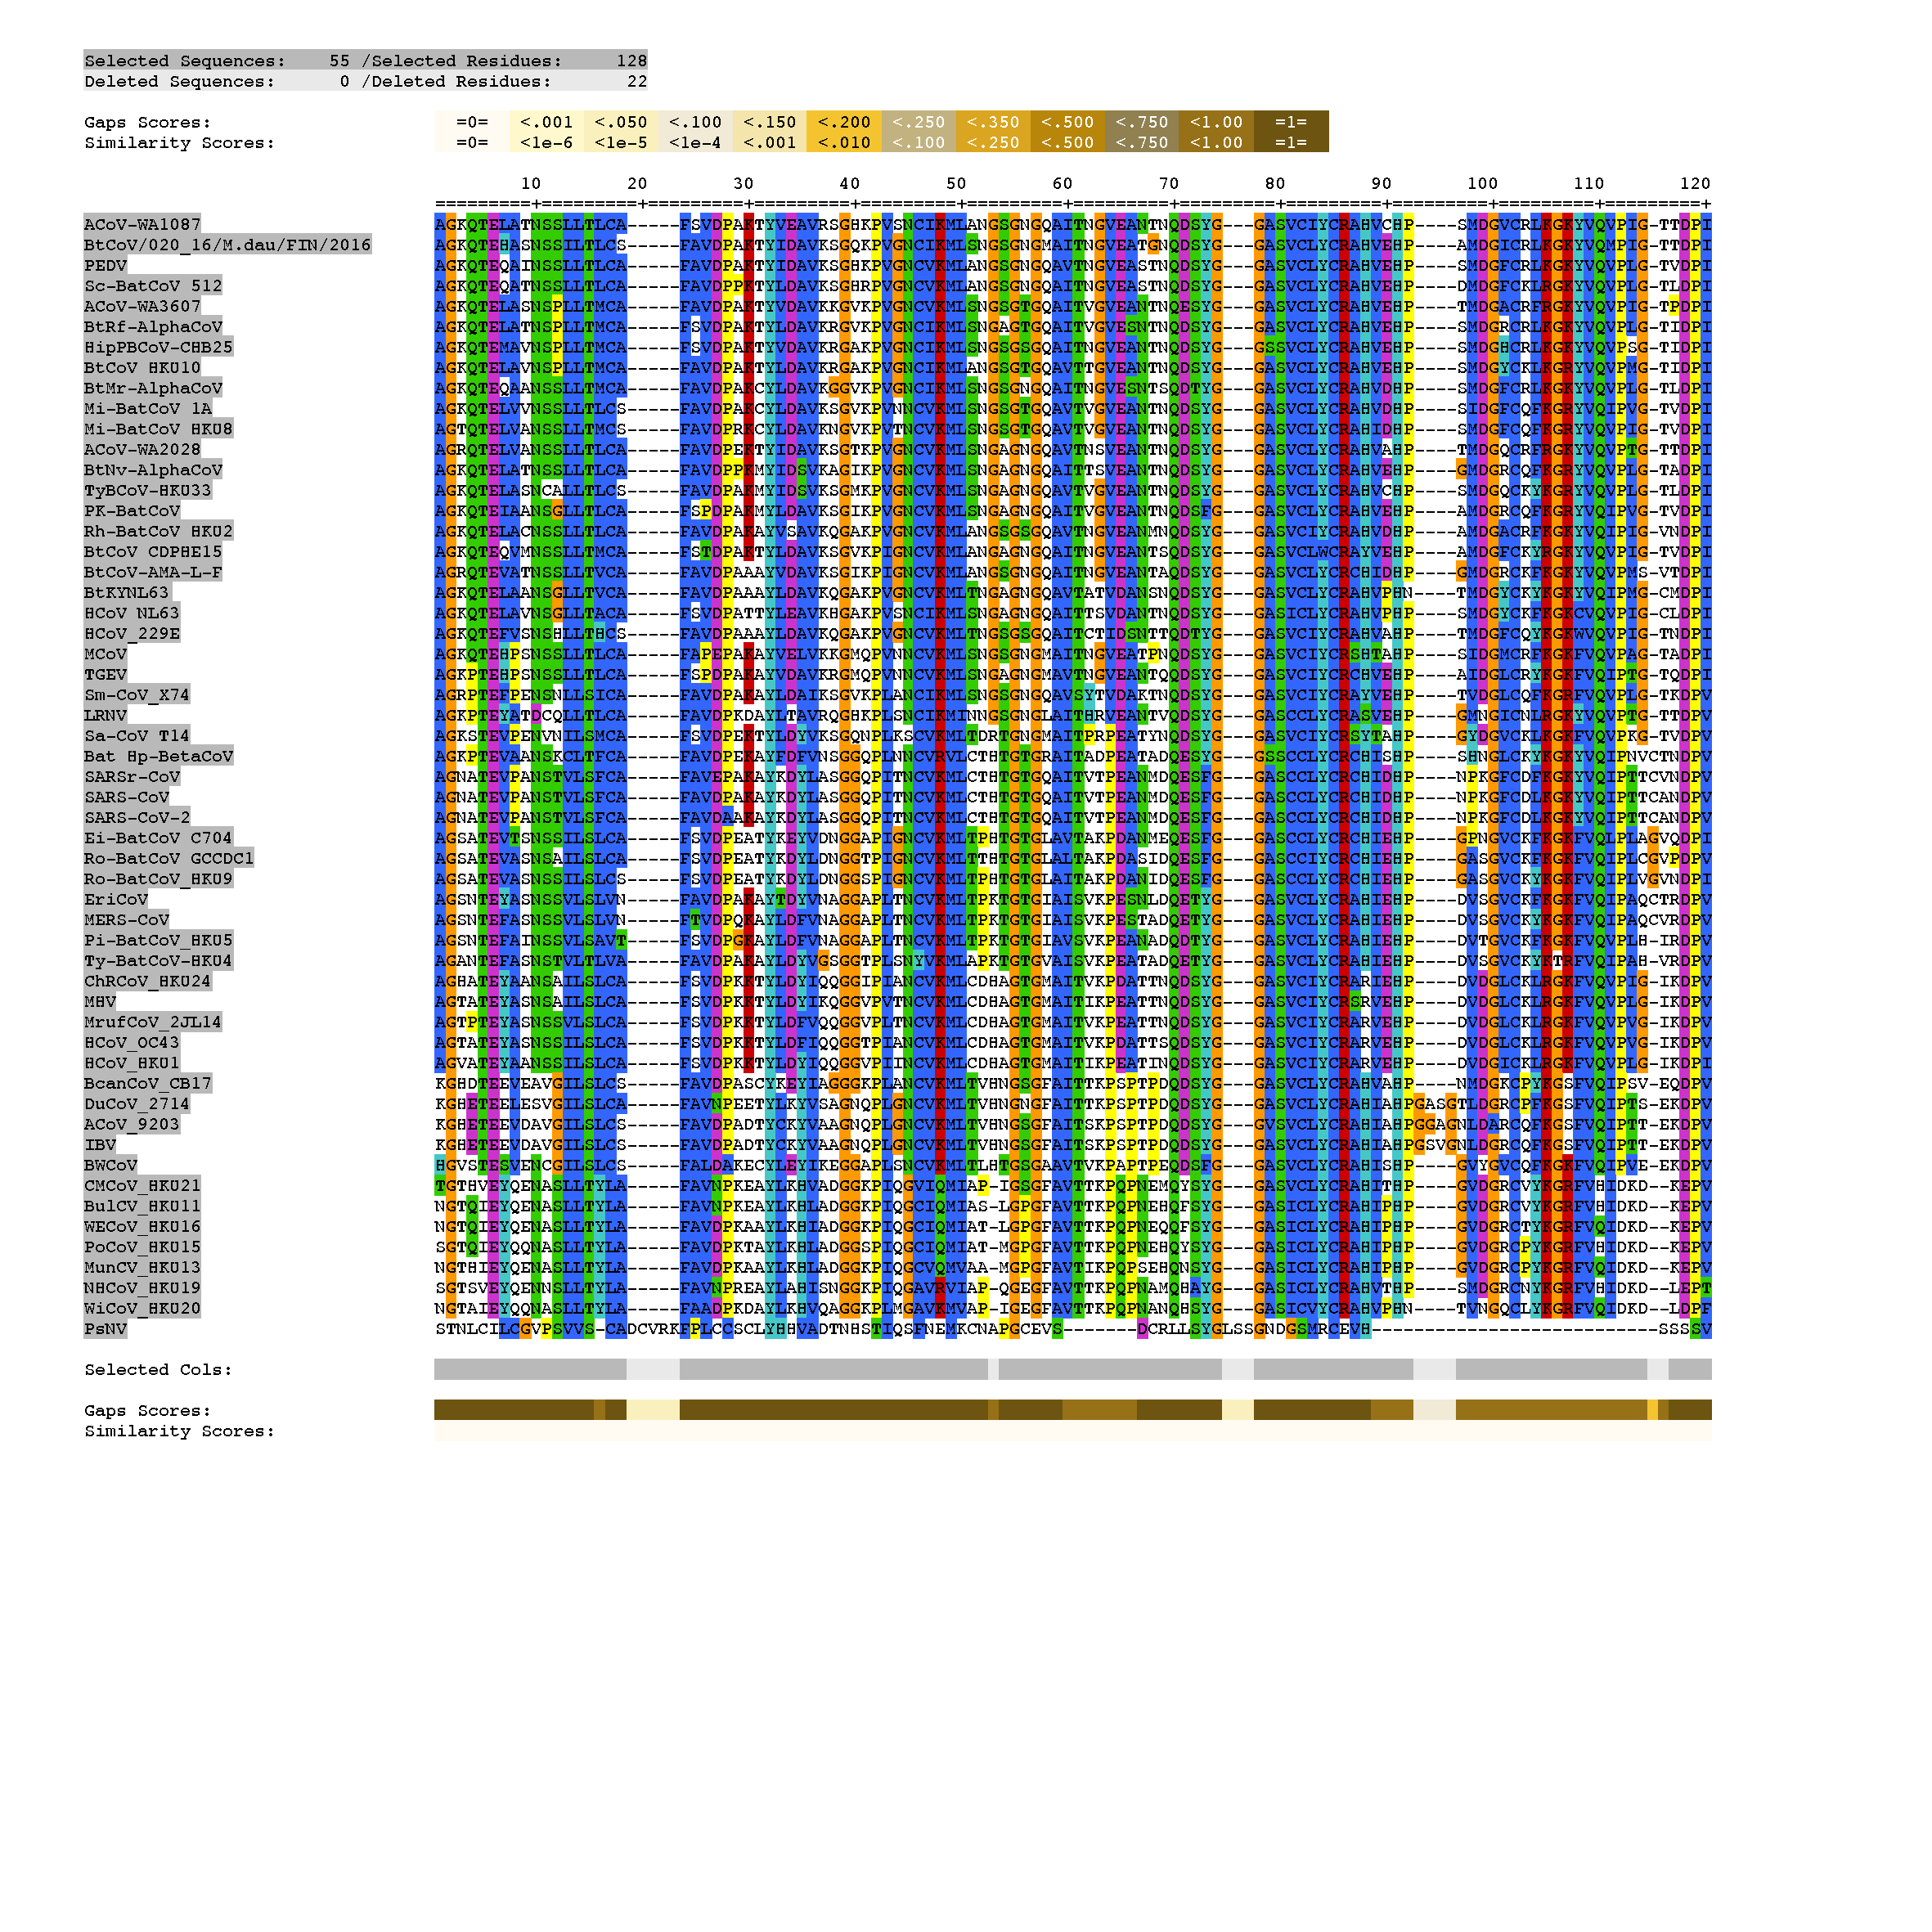
\includegraphics[width=1\textwidth]{img/fig4.pdf}
    \caption{Ejemplo de informe de los resultados de depuración de TrimAl. 
    Se muestra parcialmente el alineamiento de entrada de las proteínas 
    nsp10 con esquema de color Clustal X. Debajo, la fila de columnas 
    seleccionadas (Selected Cols) señala en gris oscuro aquellas que se 
    mantendrán en el alineamiento optimizado, y en gris claro las que 
    habrán sido eliminadas..}\label{fig:TrimAlexample}
\end{figure}

\subsubsection{Construcción de árboles filogenéticos}

Los árboles filogenéticos fueron inferidos mediante IQ-TREE.\@ Este programa 
emplea el método de máxima verosimilitud para obtener la representación más 
probable en función de los parámetros de algún modelo de evolución molecular
previamente propuesto. Se utilizó a través de la terminal de macOS mediante 
el siguiente comando:

\begin{lstlisting}[language=bash]
 iqtree2 -s TRIM_ALN_ALL_NSP10.fasta --alrt 1000 -B 1000 -m MFP -T 4
\end{lstlisting}

El comando ejecuta al programa (\lstinline!iqtree2!) para inferir un árbol 
filogenético a partir del alineamiento de secuencias depurado para esta 
finalidad (\lstinline!TRIM_ALN_ALL_NSP10.fasta!). Se aplica una prueba de 
razón de verosimilitud aproximada de 1000 réplicas (\lstinline!--alrt 1000!)
para evaluar internamente la calidad de las ramificaciones resultantes 
(\cite{guindon_new_2010}), así como una aproximación de bootstrap 
ultrarrápido de 1000 réplicas (\cite{hoang_ufboot2_2018}). Esta última es un
test estadístico ampliamente utilizado para cuantificar porcentualmente la 
robustez de los nodos de los árboles filogenéticos; aquellos marcados con 
valores más cercanos a 100 tienen alta probabilidad de ser correctos, 
mientras que aquellos que se vayan alejando de dicho valor tienen más 
probabilidad de  haber sido producidos por azar. Para seleccionar el modelo 
de evolución molecular se ejecuta una búsqueda automatizada 
(\lstinline!-m MFP!) basada en el criterio de información bayesiana, es 
decir, la selección del modelo que mejor se ajuste a los datos con la menor 
complejidad posible (\cite{kalyaanamoorthy_modelfinder_2017}). Para acelerar
la ejecución de todas estas tareas se destinaron 4 núcleos de procesamiento 
(\lstinline!-T 4!).

El comando descrito anteriormente genera varios archivos de salida que 
llevan el mismo nombre que el archivo de entrada, diferenciables por su 
extensión. Para este caso, es relevante el que contiene la estructura del 
árbol consenso generado por IQ-TREE y los valores de bootstrap para cada 
uno de sus nodos (\lstinline!TRIM_ALN_ALL_NSP10.fasta.contree!).

\subsubsection{Visualización y edición de árboles filogenéticos}

El programa IQ-TREE produce árboles no enraizados, es decir, no señalan un 
nodo basal que oriente la dirección del proceso evolutivo en el tiempo. 
Especialmente en virología, suele sacrificarse la idoneidad teórica de este 
formato forzando un nodo basal que permita visualizar resultados con una 
mayor claridad (\cite{gulyaeva_nidovirus_2021,hu_characteristics_2021,ruiz-aravena_ecology_2022}).

La visualización de los árboles fue realizada con FigTree. Este programa 
permite también editarlos mediante una selección de ajustes disponibles en 
su interfaz gráfica. A partir de los árboles no enraizados, se seleccionó al
grupo externo para presentarlos en formato rectangular. Además, se 
incluyeron los valores de Bootstrap para cada bifurcación y se exportaron 
las figuras en formato de gráficos vectoriales escalables (SVG) para su 
posterior edición en Adobe Illustrator.

\subsection{Análisis estructural de complejos proteicos}

\subsubsection{Búsqueda y selección de estructuras de referencia}

Para obtener las estructuras experimentales de los complejos proteicos 
necesarios para el análisis, se realizaron dos búsquedas en el RCSB PDB 
utilizando los términos ``SARS-CoV-2 nsp10 nsp14 complex'' y ``SARS-CoV-2 
nsp10 nsp16 complex''. Los resultados se ordenan por defecto en base a una 
puntuación de relevancia basada en la coincidencia con los términos de 
búsqueda y otros factores, como la resolución de refinamiento
(\cite{rose_rcsb_2021}).

En la \textbf{Tabla 3} se indican las estructuras tridimensionales de los 
complejos nsp10/nsp14-ExoN y nsp10/nsp16 resueltas por cristalografía de 
rayos X para SARS-CoV-2, con sus respectivos códigos de identificación 
dentro del PDB (PDB ID).

\begin{table}[H]
    \centering
    \caption{Bases de datos en línea}\label{structures}
    \scriptsize
    \setlength{\tabcolsep}{20pt} % Ajusta este valor según sea necesario
    \begin{tabularx}{\textwidth}{@{}p{7cm}p{4cm}X@{}}
    \toprule
    \textbf{Recurso} & \textbf{Fuente} & \textbf{PDB ID} \\ 
    \midrule
    Crystal structure of SARS-CoV-2 nsp10 bound to nsp14-exoribonuclease domain & (Lin et al., 2021) & \href{https://www.rcsb.org/structure/7DIY}{7DIY} \\
    1.80 Angstrom Resolution Crystal Structure of NSP16-NSP10 Complex from SARS-CoV-2 & (Rosas-Lemus et al., 2020) & \href{https://www.rcsb.org/structure/6W4H}{6W4H} \\ 
    \bottomrule
    \end{tabularx}
\end{table}

Cada estructura seleccionada fue descargada en formato de archivos del PDB 
(.pdb); un fichero de texto plano que contiene las coordenadas 
tridimensionales de cada átomo y otros datos relevantes para análisis 
estructurales (\cite{green_pdb101_2019}).

\subsubsection{Análisis de interacciones globales entre proteínas}

La visualización y los análisis de las estructuras seleccionadas fueron 
llevados a cabo con el programa ChimeraX. Este programa dispone de una 
interfaz gráfica que permite acceder a un subconjunto limitado de 
funcionalidades, así como una consola de texto que permite el manejo 
completo y preciso de la herramienta.

Para localizar los aminoácidos involucrados en la interacción 
nsp10/nsp14-ExoN de la estructura (PDB ID:7DIY), se ejecutaron tres
comandos separados secuencialmente por punto y coma:

\begin{lstlisting}[language=bash]
 sequence chain #1/A; sequence chain #1/B; interfaces #1 interfaceResidueAreaCutoff 4.5
\end{lstlisting}

Al aplicar los comandos sequence chain en la ventana principal de ChimeraX,
aparecen las secuencias aminoacídicas en formato texto de nsp10 
(\lstinline!#1/A!) y nsp14-ExoN (\lstinline!#1/B!) en ventanas secundarias. 
El comando interfaces genera en la esquina inferior derecha un diagrama de 
interacción del complejo (\lstinline!#1!) seleccionando como distancia 
límite máxima entre residuos 4.5 ángstroms 
(\lstinline!interfaceResidueAreaCutoff 4.5!) en base a las indicaciones del 
material suplementario de la publicación asociada al complejo 
(\cite{lin_crystal_2021}). Al clicar sobre el diagrama la opción 
(\lstinline!Select Contact Residues of B and A!) quedan marcados en la 
ventana principal y secundarias de color verde los aminoácidos que 
intervienen en la formación del complejo.

Estas mismas instrucciones fueron ejecutadas para la localización de los 
aminoácidos involucrados en la interacción nsp10/nsp16 de la correspondiente
estructura seleccionada (PDB ID:\@ 6W4H).

\subsubsection{Análisis de interacción de aminoácidos específicos}

Dentro del paquete de herramientas de ChimeraX, la herramienta 
\lstinline!contacts! permite identificar y visualizar los residuos 
implicados en las interacciones no covalentes de regiones concretas. Esta 
función ha sido utilizada en cada estructura de referencia con el fin de 
identificar los aminoácidos de nsp14-ExoN (PDB ID:\@ 7DIY) y nsp16 (PDB ID:\@ 
6W4H) que participan en la región de máxima interacción de nsp10 compartida 
para ambos complejos.

\subsection{Composición de figuras de resultados}

\subsubsection{Renderizado de complejos proteicos}

La herramienta save de Chimera X es utilizada para renderizar las 
visualizaciones moleculares generadas en el programa y permitir la 
exportación de los resultados en formato de imagen PNG.\@ Posteriormente, 
estas imágenes fueron montadas utilizando Adobe Illustrator para su 
presentación y análisis.

\subsubsection{Graficación de interacciones de nsp10}

Para representar en un único esquema los aminoácidos de nsp10 involucrados 
en las interacciones con nsp14-ExoN y nsp16, deducidos a partir de las 
respectivas estructuras experimentales tomadas como referencia, se utilizó 
el programa de visualización y edición de alineamientos Jalview. Bajo los 
aminoácidos de la secuencia de nsp10 se añadieron dos filas de anotaciones, 
en las que en base a viñetas de texto se señala la interacción con nsp14 y/o
nsp16. Finalmente se exportó en formato SVG para su montaje con las imágenes
de estructuras moleculares en Adobe Illustrator.

\subsubsection{Construcción de logos de secuencias}

Un logo de secuencias es una representación gráfica que permite visualizar 
la conservación de una secuencia aminoacídica (o ácidos nucleicos) a partir 
de los datos de un alineamiento (\cite{schneider_sequence_1990}). Para ello, 
se separaron las secuencias en formato FASTA de cada familia de proteínas en 
base a los cuatro géneros de la familia \textit{Orthocoronavirinae}. 
Posteriormente, se realizaron nuevos alineamientos con MAFFT para cada 
conjunto de secuencias, y se aislaron con Jalview de cada alineamiento las 
regiones de nsp14-ExoN, nsp16 y nsp10 previamente identificadas con 
ChimeraX. Los alineamientos de las regiones seleccionadas se exportaron a un
nuevo archivo FASTA para la construcción de los logos de secuencias, a 
través de la herramienta en línea WebLogo. Los gráficos obtenidos fueron 
descargados en formato SVG para su montaje en una figura conjunta con Adobe 
Illustrator.